\documentclass{ximera}
%\usepackage{todonotes}

\usepackage{tkz-euclide}
\usetikzlibrary{backgrounds} %% for boxes around graphs
\usetikzlibrary{shapes,positioning}  %% Clouds and stars
\usetkzobj{all}
\usepackage[makeroom]{cancel} %% for strike outs
%\usepackage{mathtools} %% for pretty underbrace % Breaks Ximera
\usepackage{multicol}


\newcommand{\RR}{\mathbb R}
\renewcommand{\d}{\,d}
\newcommand{\dd}[2][]{\frac{d #1}{d #2}}
\renewcommand{\l}{\ell}
\newcommand{\ddx}{\frac{d}{dx}}
\newcommand{\zeroOverZero}{$\boldsymbol{\tfrac{0}{0}}$}
\newcommand{\numOverZero}{$\boldsymbol{\tfrac{\#}{0}}$}
\newcommand{\dfn}{\textbf}
\newcommand{\eval}[1]{\bigg[ #1 \bigg]}
\renewcommand{\epsilon}{\varepsilon}
\renewcommand{\iff}{\Leftrightarrow}

\DeclareMathOperator{\arccot}{arccot}
\DeclareMathOperator{\arcsec}{arcsec}
\DeclareMathOperator{\arccsc}{arccsc}


\colorlet{textColor}{black} 
\colorlet{background}{white}
\colorlet{penColor}{blue!50!black} % Color of a curve in a plot
\colorlet{penColor2}{red!50!black}% Color of a curve in a plot
\colorlet{penColor3}{red!50!blue} % Color of a curve in a plot
\colorlet{penColor4}{green!50!black} % Color of a curve in a plot
\colorlet{penColor5}{orange!80!black} % Color of a curve in a plot
                                      \colorlet{fill1}{blue!50!black!20} % Color of fill in a plot
\colorlet{fill2}{blue!10} % Color of fill in a plot
\colorlet{fillp}{fill1} % Color of positive area
\colorlet{filln}{red!50!black!20} % Color of negative area
\colorlet{gridColor}{gray!50} % Color of grid in a plot

\pgfmathdeclarefunction{gauss}{2}{% gives gaussian
  \pgfmathparse{1/(#2*sqrt(2*pi))*exp(-((x-#1)^2)/(2*#2^2))}%
}



\newcommand{\fullwidth}{}
\newcommand{\normalwidth}{}



%% makes a snazzy t-chart for evaluating functions
\newenvironment{tchart}{\rowcolors{2}{}{background!90!textColor}\array}{\endarray}

%%This is to help with formatting on future title pages.
\newenvironment{sectionOutcomes}{}{} 

\author{Emma Smith Zbarsky}
\license{Creative Commons Attribution 3.0 Unported}
\acknowledgement{https://quadbase.org/questions/q13632v1}
\begin{document}

\begin{exercise}

Calculate

*$f(.5) =$

*$f(.1) = $

*$f(.01) = $

*$f(.001) = $

*$f(.0001) = $

*$f(-.0001) = $

*$f(-.001) = $

*$f(-.01) = $

*$f(-.1) = $

*$f(-.5)= $


\begin{hint}
Use a spreadsheet program to calculate the requested values.
\end{hint}


\begin{hint}
\begin{image}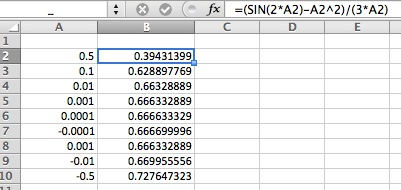
\includegraphics{numerical-limit-practice.jpg}\end{image}
\end{hint}


\begin{multipleChoice}
\choice[correct]{*$f(.5) = 0.39431399$

*$f(.1) = 0.628897769$

*$f(.01) = 0.66328889$

*$f(.001) = 0.666332889$

*$f(.0001) = 0.666633329$

*$f(-.0001) = 0.666699996$

*$f(-.001) = 0.666999556$

*$f(-.01) = 0.669955556$

*$f(-.1) = 0.695564436$

*$f(-.5)= 0.727647323$}
\choice{*$f(.5) = 0.727647323$

*$f(.1) = 0.695564436$

*$f(.01) = 0.669955556$

*$f(.001) = 0.666999556$

*$f(.0001) = 0.666699996$

*$f(-.0001) = 0.666633329$

*$f(-.001) = 0.666332889$

*$f(-.01) = 0.66328889$

*$f(-.1) = 0.628897769$

*$f(-.5)= 0.39431399$}
\choice{*$f(.5) = -0.139798463$

*$f(.1) = -0.033111407$

*$f(.01) = -0.003333111$

*$f(.001) = -0.000333333$

*$f(.0001) = -3.33333E-05$

*$f(-.0001) = 3.33333E-05$

*$f(-.001) = 0.000333333$

*$f(-.01) = 0.003333111$

*$f(-.1) = 0.033111407$

*$f(-.5)= 0.139798463$}
\end{multipleChoice}

\end{exercise}
\end{document}
